\documentclass{article}

\usepackage[spanish]{babel}
\usepackage[utf8]{inputenc}
\usepackage{fancyhdr}
\usepackage{extramarks}
\usepackage{amsmath}
\usepackage{amsthm}
\usepackage{amsfonts}
\usepackage{tikz}
\usepackage{algorithm}
\usepackage{algpseudocode}
\usepackage{hyperref}
\usepackage{graphicx}
\usepackage{float}
\usepackage{natbib}
\usepackage{subcaption}

\usetikzlibrary{automata,positioning}

%
% Basic Document Settings
%

\topmargin=-0.45in
\evensidemargin=0in
\oddsidemargin=0in
\textwidth=6.5in
\textheight=9.0in
\headsep=0.25in

\linespread{1.1}

\pagestyle{fancy}
\lhead{\hmwkAuthorName}

\setlength{\headheight}{35pt}

\chead{
	\parbox{0.8\textwidth}{
		\centering
		\hmwkClass\ (\hmwkClassInstructor)\\
		\hmwkTitle
}}

\rhead{\firstxmark}
\lfoot{\lastxmark}
\cfoot{\thepage}

\renewcommand\headrulewidth{0.4pt}
\renewcommand\footrulewidth{0.4pt}

\setlength\parindent{0pt}

%
% Create Problem Sections
%

\newcommand{\enterProblemHeader}[2]{
	\nobreak\extramarks{}{Problema {#1} continúa en la sig pág\ldots}\nobreak{}
	\nobreak\extramarks{Problema \arabic{#1} (continúa)}{Problema \arabic{#1} continúa en la sig pág\ldots}\nobreak{}
}

\newcommand{\exitProblemHeader}[2]{
	\nobreak\extramarks{Problema \arabic{#1}}{Problema \arabic{#1} continúa en la sig pág\ldots}\nobreak{}
	\stepcounter{#1}
	\nobreak\extramarks{Problema \arabic{#1}}{}\nobreak{}
}

\setcounter{secnumdepth}{0}
\newcounter{partCounter}
\newcounter{homeworkProblemCounter}
\setcounter{homeworkProblemCounter}{6}
\nobreak\extramarks{Problema \arabic{homeworkProblemCounter}}{}\nobreak{}

%
% Homework Problem Environment
%
% This environment takes an optional argument. When given, it will adjust the
% problem counter. This is useful for when the problems given for your
% assignment aren't sequential. See the last 3 problems of this template for an
% example.
%
\newenvironment{homeworkProblem}[2][-1]{
	\ifnum#1>0
	\setcounter{homeworkProblemCounter}{#1}
	\fi
	\def\currentProblemTitle{#2}
	\section{Problema \arabic{homeworkProblemCounter}: #2}
	\setcounter{partCounter}{1}
	\enterProblemHeader{homeworkProblemCounter}{#2}
}{
	\exitProblemHeader{homeworkProblemCounter}{\currentProblemTitle}
}
%
% Homework Details
%   - Title
%   - Due date
%   - Class
%   - Section/Time
%   - Instructor
%   - Author
%

\newcommand{\hmwkTitle}{Descomposición Celular Exacta para una barra L\ \#6}
\newcommand{\hmwkDueDate}{21 de mayo de 2026}
\newcommand{\hmwkClass}{Planificación de movimientos de robots}
\newcommand{\hmwkClassInstructor}{Rafael Murrieta Cid}
\newcommand{\hmwkAuthorName}{\textbf{Andrés Alemán}}

%
% Title Page
%

\title{
	\vspace{2in}
	\textmd{\textbf{\hmwkClass:\ \hmwkTitle}}\\
	\normalsize\vspace{0.1in}\small{Due\ on\ \hmwkDueDate}\\
	\vspace{0.1in}\large{\textit{\hmwkClassInstructor}}
	\vspace{3in}
}

\author{\hmwkAuthorName}
\date{}

\renewcommand{\part}[1]{\textbf{\large Parte \Alph{partCounter}}\stepcounter{partCounter}\\}

%
% Various Helper Commands
%

% Useful for algorithms
\newcommand{\alg}[1]{\textsc{\bfseries \footnotesize #1}}

% For derivatives
\newcommand{\deriv}[1]{\frac{\mathrm{d}}{\mathrm{d}x} (#1)}

% For partial derivatives
\newcommand{\pderiv}[2]{\frac{\partial}{\partial #1} (#2)}

% Integral dx
\newcommand{\dx}{\mathrm{d}x}

% Alias for the Solution section header
\newcommand{\solution}{\textbf{\large Solución}}

% Probability commands: Expectation, Variance, Covariance, Bias
\newcommand{\E}{\mathrm{E}}
\newcommand{\Var}{\mathrm{Var}}
\newcommand{\Cov}{\mathrm{Cov}}
\newcommand{\Bias}{\mathrm{Bias}}

\begin{document}
	
%	\maketitle
	
%	\pagebreak
	
	\begin{homeworkProblem}{Descomposición Celular Exacta para una barra L}
	
	\section{Introducción}
	El problema de la planificación de movimientos para un robot tipo barra (o \textit{rod/ladder}) en el plano consiste en encontrar una trayectoria continua en su espacio de configuración $C$ que evite colisiones con los obstáculos. A diferencia de un robot puntual, una barra de longitud $L$ posee dimensiones físicas que restringen tanto su posición como su orientación \cite{Latombe1991}. El método de \textbf{Descomposición Celular Exacta} aborda este problema dividiendo el espacio libre ($C_{free}$) en una colección finita de regiones no sobrepuestas llamadas \textbf{celdas}. La conectividad de estas celdas se representa mediante un \textbf{grafo de conectividad}, donde cada nodo es una celda y cada arista indica que el robot puede transitar físicamente entre ellas \cite{Latombe1991}. En este trabajo, analizaremos un corredor recto de ancho $\ell$ y una barra de longitud $L$, evaluando la topología del grafo resultante.
	
	\section{Marco Teórico y Notación}
	
	\subsection{Espacio de Configuración (C-Space)}
	Para un robot barra $A$ en el plano, el espacio de configuración se define como $C = \mathbb{R}^2 \times S^1$. Una configuración $q = (x, y, \theta)$ especifica la posición del punto de referencia $P$ y su orientación $\theta \in [0, 2\pi)$ \cite{Latombe1991}.
	
	\subsection{Curvas Críticas y Regiones No Críticas}
	Las \textbf{curvas críticas} marcan dónde la estructura de las orientaciones libres cambia cualitativamente. Para los siguientes ejercicios, la curva fundamental de interés es la \textbf{Tipo 1}:
	\begin{itemize}
		\item \textbf{Curva Tipo 1:} Es un segmento de recta paralelo a un borde del obstáculo situado a una distancia $L$. Define el límite donde el punto $P$ permite que la barra rote sin chocar con la pared.
	\end{itemize}
	
	Una \textbf{región no crítica} $R$ es un subconjunto del plano $xy$ delimitado por estas curvas, donde el conjunto de ángulos libres $F(x, y)$ se mantiene estructuralmente constante \cite{Latombe1991}.
	
	\subsection{Definición de Celdas y Stops}
	Siguiendo la notación de Latombe, una celda se define como el trío:
	\begin{equation}
		C_i = (R, s_1, s_2)
	\end{equation}
	Donde $s_1$ y $s_2$ son los \textbf{stops} o bordes de obstáculos que limitan el intervalo de rotación \cite{Latombe1991}. El símbolo $\Omega$ indica rotación libre de $360^\circ$ \cite{Murrieta2026}.
	
	\section{Análisis de Casos según la Proporción $L$ y $\ell$}
	
	% --- CASO 1 ---
	\subsection{Caso 1: $L < \ell$ (Barra corta)}
	En este escenario, la longitud de la barra $L$ es menor al ancho del corredor $\ell$. Esto permite la existencia de regiones donde el robot puede realizar una rotación completa de $360^\circ$ sin colisionar con las paredes.
	
	\textbf{Análisis Geométrico:} Aparecen dos curvas críticas de \textbf{Tipo 1} dentro del corredor, situadas a una distancia $L$ de cada pared ($W_1$ superior y $W_2$ inferior). Esto divide el espacio de traslación en tres regiones no críticas:
	\begin{itemize}
		\item $R_0$: Región central donde el punto de referencia $P$ está a distancia $> L$ de ambas paredes.
		\item $R_1$: franja superior cerca de $W_1$.
		\item $R_2$: franja inferior cerca de $W_2$.
	\end{itemize}
	
	\begin{figure}[htbp]
		\centering
		\begin{subfigure}{0.48\textwidth}
			\centering
			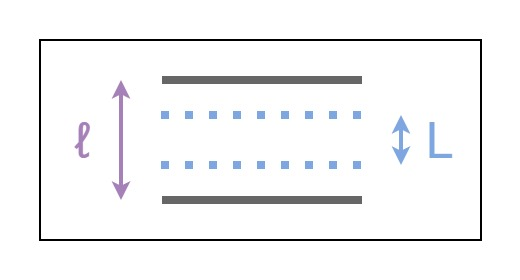
\includegraphics[width=\linewidth]{corredor_caso1.jpg}
			\caption{Referencia del corredor y la barra ($L < \ell$).}
		\end{subfigure}
		\hfill
		\begin{subfigure}{0.48\textwidth}
			\centering
			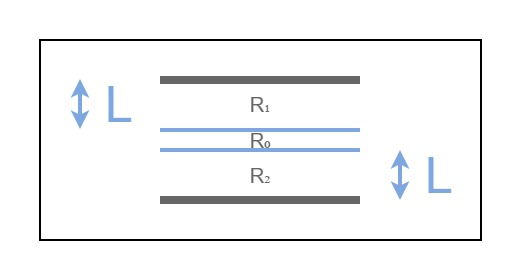
\includegraphics[width=\linewidth]{regiones_caso1.jpg}
			\caption{Curvas Tipo 1 y regiones no críticas resultantes.}
		\end{subfigure}
		\caption{Caso 1: configuración y análisis geométrico.}
	\end{figure}
	
	\medskip
		
	\textbf{Definición de Celdas y Grafo:} 
	En $R_0$, el conjunto de orientaciones libres es $F(x,y) = [0, 2\pi)$, por lo que la celda se define como $C_0 = (R_0, \Omega, \Omega)$. En las regiones laterales, la rotación está limitada por el contacto con la pared adyacente. El grafo resultante es \textbf{conectado}, permitiendo al robot transitar de una pared a otra y cambiar su orientación completamente al pasar por el centro.
	
	\medskip

	\begin{figure}[H]
		\centering
		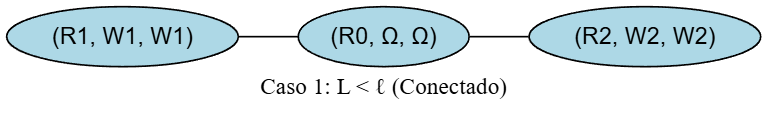
\includegraphics[width=0.7\textwidth]{grafo_caso1.png}
		\caption{Grafo de conectividad (Estructura conectada).}
	\end{figure}
	
	% --- CASO 2 ---
	\subsection{Caso 2: $L > 2\ell$ (Barra muy larga)}
	Cuando la barra es considerablemente más larga que el ancho del corredor ($L > 2\ell$), las curvas críticas de Tipo 1 quedan fuera del espacio físico del corredor.
	
	\textbf{Análisis Geométrico:} Todo el interior del corredor se convierte en una única región no crítica $R_0$. Sin embargo, debido a que $L > \ell$, la barra \textbf{nunca puede alcanzar una orientación vertical} ($\theta = 90^\circ$ o $270^\circ$) sin colisionar con ambas paredes simultáneamente.
	
	\begin{figure}[H]
		\centering
		\begin{subfigure}{0.48\textwidth}
			\centering
			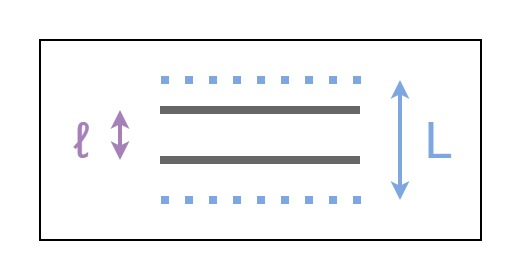
\includegraphics[width=\linewidth]{corredor_caso2.jpg}
			\caption{Referencia del corredor y la barra ($L > 2\ell$).}
		\end{subfigure}
		\hfill
		\begin{subfigure}{0.48\textwidth}
			\centering
			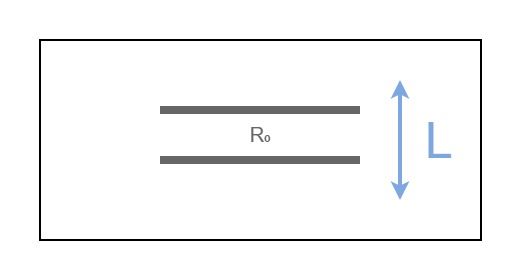
\includegraphics[width=\linewidth]{regiones_caso2.jpg}
			\caption{Región única $R_0$ (Curvas críticas fuera del corredor).}
		\end{subfigure}
		\caption{Caso 2: configuración y análisis geométrico.}
	\end{figure}
	
	\medskip
	
	\textbf{Definición de Celdas y Grafo:} El espacio de configuraciones libres $C_{free}$ se fragmenta en dos componentes disjuntas. Existen dos intervalos de ángulos libres que no se solapan, representados por las celdas:
	\begin{itemize}
		\item $C_{der} = (R_0, W_1, W_2)$: La barra apunta hacia la derecha.
		\item $C_{izq} = (R_0, W_2, W_1)$: La barra apunta hacia la izquierda.
	\end{itemize}
	El grafo está \textbf{desconectado}, lo que indica que el robot puede trasladarse a lo largo del corredor pero es incapaz de girar para invertir su sentido de marcha.
	
	\begin{figure}[H]
		\centering
		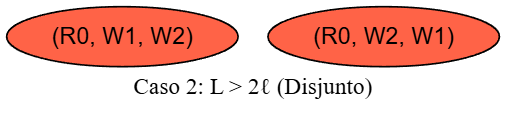
\includegraphics[width=0.5\textwidth]{grafo_caso2.png}
		\caption{Grafo de conectividad (Dos componentes disjuntas).}
	\end{figure}
	
	% --- CASO 3 ---
	\subsection{Caso 3: $\ell < L < 2\ell$ (Barra de longitud intermedia)}
	En un corredor recto infinito, este caso es topológicamente equivalente al Caso 2. Aunque la barra es más corta que en el ejercicio anterior, el hecho de que $L$ siga siendo mayor que el ancho $\ell$ del corredor impide mecánicamente la rotación completa.
	
	\textbf{Análisis Geométrico:} Al igual que en el caso anterior, las curvas de Tipo 1 no intersectan el corredor libre. El punto de referencia $P$ siempre se encuentra a una distancia menor a $L$ de ambas paredes, lo que restringe el intervalo de ángulos libres $F(x,y)$ a dos sectores opuestos.
	
	\begin{figure}[htbp]
		\centering
		\begin{subfigure}{0.48\textwidth}
			\centering
			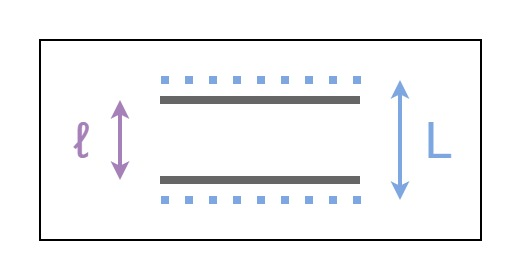
\includegraphics[width=\linewidth]{corredor_caso3.jpg}
			\caption{Referencia del corredor y la barra ($\ell < L < 2\ell$).}
		\end{subfigure}
		\hfill
		\begin{subfigure}{0.48\textwidth}
			\centering
			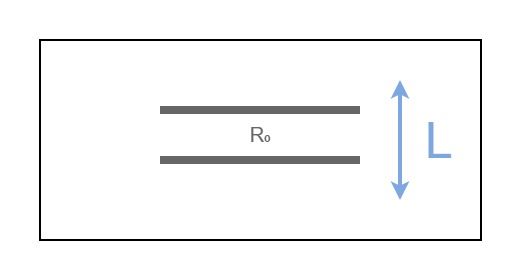
\includegraphics[width=\linewidth]{regiones_caso3.jpg}
			\caption{Análisis de regiones para longitud intermedia.}
		\end{subfigure}
		\caption{Caso 3: configuración y análisis geométrico.}
	\end{figure}
		
	\medskip
	
	\textbf{Definición de Celdas y Grafo:} Se mantienen las mismas celdas disjuntas $C_{der}$ y $C_{izq}$ en la región $R_0$. No existe ningún "canal" o secuencia de celdas que permita pasar de una orientación a otra. La importancia de la medida $2\ell$ suele ser relevante solo en presencia de esquinas o intersecciones, donde permitiría maniobras que aquí son imposibles.
			
	\begin{figure}[H]
		\centering
		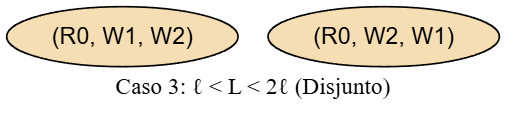
\includegraphics[width=0.5\textwidth]{grafo_caso3.png}
		\caption{Grafo de conectividad (Desconectado).}
	\end{figure}
	
				
	\end{homeworkProblem}
	
	\pagebreak
	\bibliographystyle{plainnat}
	\bibliography{biblio}
\end{document}
